\chapter {System Design and Analysis}
\noindent
\rule{\textwidth}{0.4pt}

\begin{center}
\begin{minipage}{0.8\textwidth}
\textit{Chapter 3 presents the system design and analysis of the CodeRank platform. It first defines the stakeholders, functional requirements, and non-functional requirements, followed by the major use cases of the system. The chapter then describes the architecture, submission evaluation flow, ranking mechanism, database schema, and chatbot design that support the platform's core functionality.}
\end{minipage}

\end{center}

\section{Requirement analysis}
\subsection{Stakeholders}
In any software system, understanding the stakeholders is essential for defining responsibilities, ensuring smooth operation, and aligning the platform with user needs. This project identifies three main groups of stakeholders, each playing a critical role in the development, management, and effective use of the platform. The following sections describe these groups in detail: Primary Users, Moderators, and Superadmin.
\begin{enumerate}
    \item \textbf{Primary Users}\\
    Primary users consist of students, programming contestants, and job seekers who utilize the platform to enhance their coding abilities and evaluate their technical proficiency. These users engage with the system by practicing programming challenges, submitting solutions for automated evaluation, and participating in online contests that allow them to monitor their progress and compare performance with peers. Additionally, they may take part in discussion forums to exchange ideas and seek guidance. The platform also provides access to an integrated virtual assistant designed to support interview preparation, enabling users to develop both competitive and career-readiness skills.
    \item \textbf{Moderators}\\
    Moderators serve as the quality control and management layer of the platform. Their responsibilities include reviewing problem statements, validating test cases, and monitoring ongoing contests to ensure fairness and a seamless experience for all participants. Moreover, moderators oversee the integrity of the system by detecting plagiarism, resolving disputes, and upholding community standards within discussion forums. Their involvement is essential for maintaining a trustworthy, transparent, and academically honest environment.
    \item \textbf{Superadmin}\\
    The Superadmin holds the highest level of authority within the system and is responsible for overarching platform management. In addition to performing all moderator functions, the Superadmin oversees system-wide operations, configures platform policies, and supervises both moderators and regular users. Their core duties include creating and managing moderator accounts, managing roles, addressing escalated issues, and monitoring system performance through analytics and operational metrics. This role ensures that the platform remains stable, secure, and aligned with organizational objectives.
\end{enumerate}

\subsection{Functional requirements}
\vspace{0.3cm}
\noindent \textbf{\Large Primary Users}
\vspace{0.3cm}
\begin{enumerate}[label=\arabic*.]
    \item \textit{Authentication:}
        \begin{itemize}
            \item The system shall allow users to create an account using email and password or third-party authentication providers (e.g., Google, GitHub).
            \item The system shall support secure login and logout functionality.
            \item The system shall provide password recovery and reset options.
            \item The system shall enforce role-based access control to differentiate between standard users, moderators, and superadmins.
        \end{itemize}
    \item \textit{Problem Solving and Submission:}
        \begin{itemize}
            \item The system shall allow users to browse and search algorithmic problems by difficulty, topic, tags, and status (solved, attempted).
            \item The system shall provide an integrated code editor supporting multiple programming languages (C++, Java, Python), enabling users to write, compile, and execute their code against provided example test cases.
            \item The system shall display immediate feedback on submitted solutions, indicating success/failure, execution time, memory usage, and specific error messages (e.g., Wrong Answer, Time Limit Exceeded, Runtime Error).
            \item The system shall allow users to view their past submissions and their results.
        \end{itemize}
    \item \textit{Contest Participation:}
        \begin{itemize}
            \item The system shall enable users to create or participate in online programming contests. In case the users want to create an online contest, they can enforce the contest rules, such as time limits per problem and penalty for incorrect submissions.
            \item The system shall display a leaderboard after the contests finish.
        \end{itemize}
    \item \textit{Community forum:}
        \begin{itemize}
            \item The system shall provide a shared discussion forum where users can exchange ideas, ask questions, and discuss solutions for all problems, similar to a general online community forum.
            \item The system shall allow users to upvote/downvote comments and report inappropriate content.
        \end{itemize}
    \item \textit{Ranking System:}
        \begin{itemize}
            \item The system shall assign points to users upon successfully solving problems, with points varying according to the difficulty of each problem.
            \item The ranking system shall update user scores and global rankings every 15 minutes, reflecting users’ latest achievements and progress.
        \end{itemize}
    \item \textit{Interview Preparation (Virtual Assistant):}
        \begin{itemize}
            \item The system shall offer a virtual assistant feature for practicing interview questions (e.g., mock interviews with predefined scenarios).
            \item The system shall provide hints and feedback on interview responses.
        \end{itemize}
\end{enumerate}
\vspace{0.3cm}
\noindent \textbf{\Large Moderators}
\vspace{0.3cm}
\begin{enumerate}
    \item \textit{Problems Management:}
        \begin{itemize}
            \item The system shall allow moderators to create, edit, and publish new algorithmic problems.
            \item The system shall enable moderators to define problem statements, input/output formats, constraints, and sample test cases.
            \item The system shall allow moderators to upload and manage hidden test cases for problem evaluation.
        \end{itemize}
    \item \textit{Contest Management:}
        \begin{itemize}
            \item The system shall allow moderators to receive and review requests from users for creating new contests. Moderators shall have the ability to either approve or reject these contest creation demands, providing a reason for rejection if applicable. Upon approval, the system shall notify the requesting user and enable the moderator to proceed with configuring and publishing the contest.
        \end{itemize}
    \item \textit{Community Moderation:}
        \begin{itemize}
            \item The system shall allow moderators to review and manage content in discussion forums, including deleting inappropriate posts or comments.
            \item The system shall enable moderators to warn or ban users who violate community guidelines.
        \end{itemize}
\end{enumerate}
\vspace{0.3cm}
\noindent \textbf{\Large Superadmin}
\vspace{0.3cm}\\
The Superadmin shall possess all the functional capabilities and permissions granted to a moderator.
\begin{enumerate}
    \item \textit{User and Moderator Account Management:}
        \begin{itemize}
            \item The system shall allow the Superadmin to create, edit, suspend, and delete user and moderator accounts.
            \item The system shall enable moderators to warn or ban users who violate community guidelines.
        \end{itemize}
\end{enumerate}

\subsection{Non-functional requirements}
\noindent \textit{Performance:} The system shall support at least 1,000 concurrent users while maintaining minimal latency during contests. Code submissions must be evaluated and feedback returned within 3 seconds for standard test cases, ensuring a responsive and smooth user experience.\\

\noindent \textit{Scalability:} The system shall be designed to support horizontal scaling, allowing it to handle increasing numbers of users and higher workloads by adding additional servers or computational resources as needed.\\

\noindent \textit{Reliability:} The system shall maintain high availability, particularly during contests and peak usage periods. Mechanisms for fault tolerance and recovery shall be implemented to minimize downtime and ensure continuous operation.\\

\noindent \textit{Security:} The system shall safeguard user accounts, code submissions, and any sensitive data (including payment information) through industry-standard security measures, such as encryption, secure authentication, and role-based access control.\\

\noindent \textit{Usability:} The system shall provide an intuitive and user-friendly interface suitable for both beginners and advanced users. Users should be able to quickly locate problems by difficulty or topic, join contests with minimal steps, and utilize the integrated code editor without additional setup.\\

\noindent \textit{Maintainability:} The system shall be designed for ease of maintenance, allowing developers to update features, fix bugs, and enhance functionality with minimal effort and disruption.\\

\noindent \textit{Internationalization \& Localization:} The system shall support multiple languages and provide seamless switching between them, ensuring accessibility and usability for a diverse, global user base.
\section{Use Cases}
\subsection{General Use Case}

\begin{figure}[h!]
    \centering
    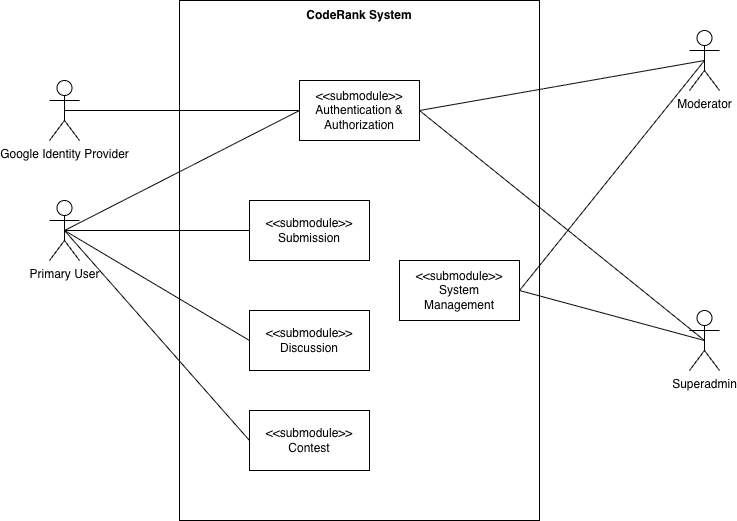
\includegraphics[width=1\textwidth]{Contents/Chapter 3/Usecase/Images/GeneralUsecase.png}
    \vspace{0.6cm}
    \caption{General Use Case}
\end{figure}


Our system contains 5 main submodules:
\begin{itemize}
    \item \textbf{Authentication \& Authorization}: Responsible for managing secure login and enforces Role-Based Access Control for 3 types of user.
    \item \textbf{Discussion}: Facilitates community interaction, allowing primary users to share solutions and ask questions related to problems. 
    \item \textbf{System Management}: The administrative interface used by Moderator and Superadmin to manage the problem creation, test cases, contests management and global user accounts.
Contest: Enables timed, high-stakes programming events with real-time ranking and automated leaderboards.
    \item \textbf{Submission}: This core module handles the presentation of the coding challenge and the automatic evaluation of the user's submitted solution.
\end{itemize}

\subsection{Use-case diagrams for each submodule}

\begin{figure}[h!]
    \centering
    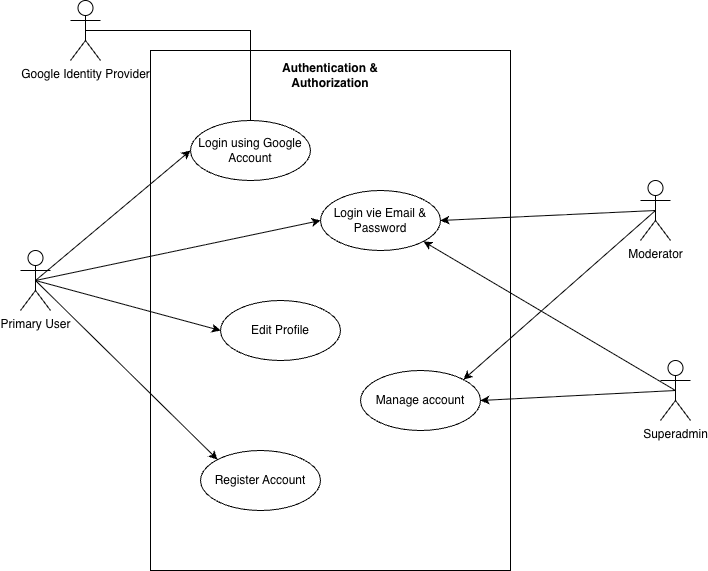
\includegraphics[width=1\textwidth]{Contents/Chapter 3/Usecase/Images/GeneralUsecase-Authentication.drawio.png}
    \vspace{0.6cm}
    \caption{Authentication \& Authorization Use Case}
\end{figure}
This submodule serves as the primary security gate for the entire system. Its core responsibility is to handle all user authentication (logging in) and authorization (managing access rights). This is crucial for protecting users' personal information, ensuring data privacy, and securing sensitive actions within the platform. By strictly controlling access, the module prevents unauthorized entry and maintains system integrity.
For user convenience, we offer diverse login methods:
\begin{itemize}
    \item Primary Users can log in quickly using their Google Account or use the traditional \textbf{Email \& Password} method.
    \item However, for privileged administrative roles—the Moderator and the Superadmin—access is strictly limited to the Login via \textbf{Email \& Password} method to enforce heightened security and traceability for system management functions.
\end{itemize}

All users retain standard account management capabilities, including registering a new account and changing their password.

\begin{figure}[h!]
    \centering
    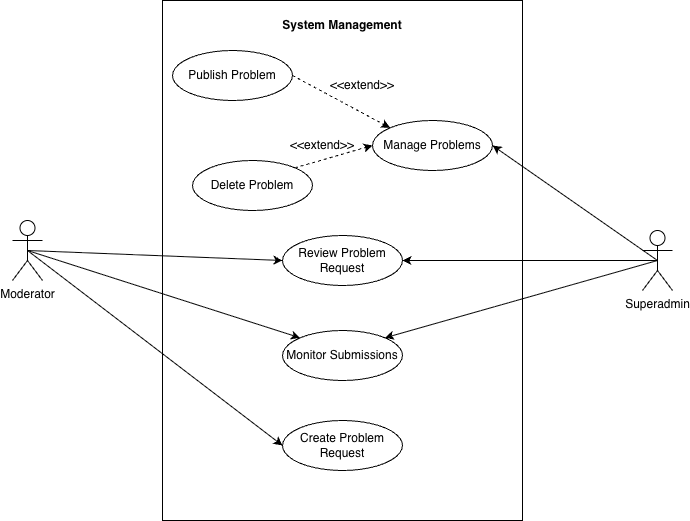
\includegraphics[width=1\textwidth]{Contents/Chapter 3/Usecase/Images/GeneralUsecase-SystemManagement.drawio.png}
    \vspace{0.6cm}
    \caption{System Management Use Case}
\end{figure}
The \textbf{System Management submodule} is the administrative dashboard used exclusively by the \textbf{Moderator} and \textbf{Superadmin} roles to control the content and operation of the platform.
\begin{itemize}
    \item \textbf{Problem Management}: Only Superadmin is enabled to manage problems directly (create, modify, delete) without reviewing steps
    \item \textbf{Content Workflow}: The Moderator initiates a Create Problem Request, and both the Moderator and Superadmin review problem requests before they go live.
    \item \textbf{Quality Control}: Both roles Monitor Submissions to track user activity, diagnose potential grading issues, and ensure fair play.
\end{itemize}
\clearpage

\begin{figure}[h!]
    \centering
    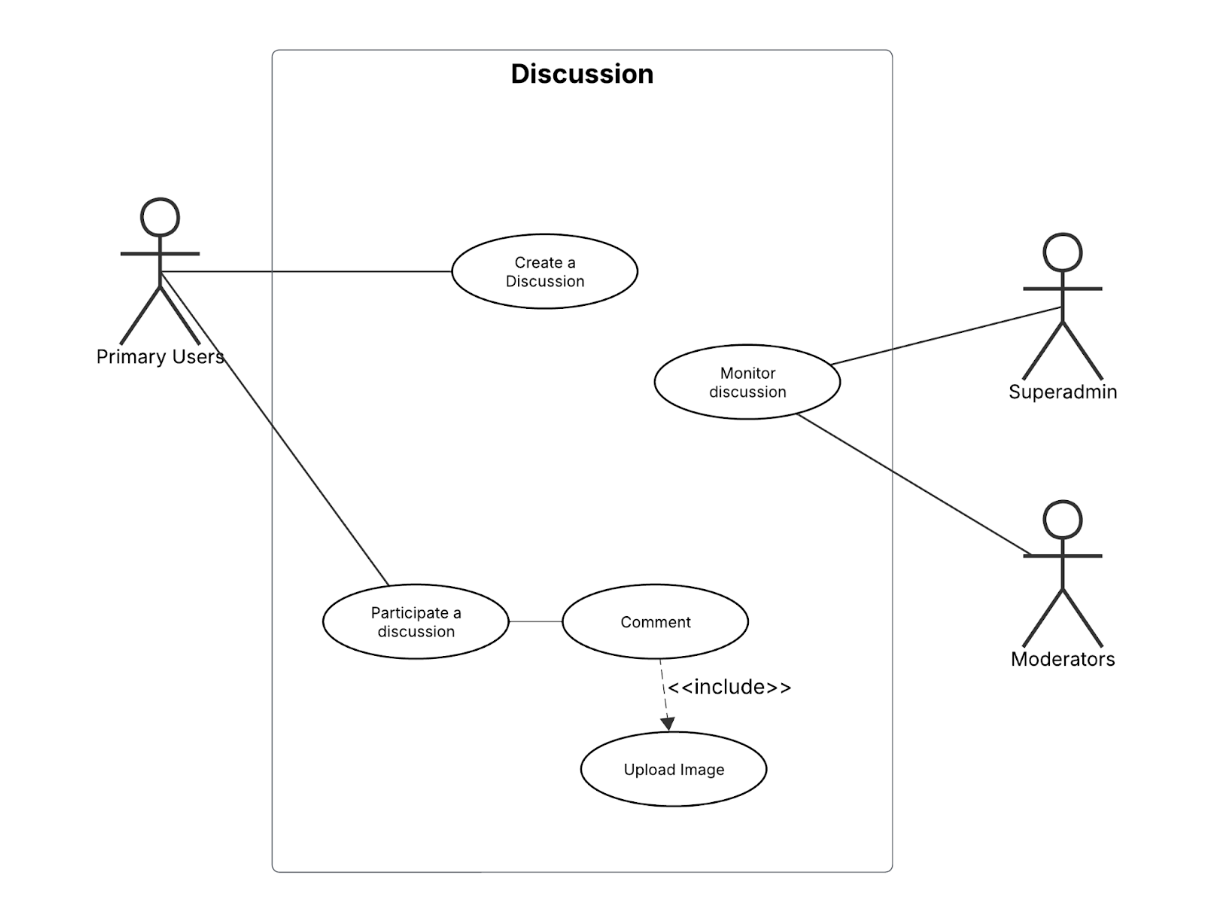
\includegraphics[width=1\textwidth]{Contents/Chapter 3/Usecase/Images/Discussion.png}
    \vspace{0.6cm}
    \caption{Discussion Use Case}
\end{figure}
The \textbf{Discussion submodule} helps make CodeRank a friendly and interactive community where users can learn from each other. With the Create Discussion feature, users can start new discussion threads about coding problems, programming ideas, or any tech-related topic. After a thread is created, others can join in by commenting on that thread. Comments can include rich content, such as images added, making explanations clearer and easier to follow.
To ensure that discussions remain constructive and aligned with community guidelines, the submodule integrates essential administrative controls. Both the Superadmin and Moderators utilize the Monitor Discussion function to oversee user activity, identify and address inappropriate content, and uphold the platform’s community standards. 

\clearpage

\begin{figure}[h!]
    \centering
    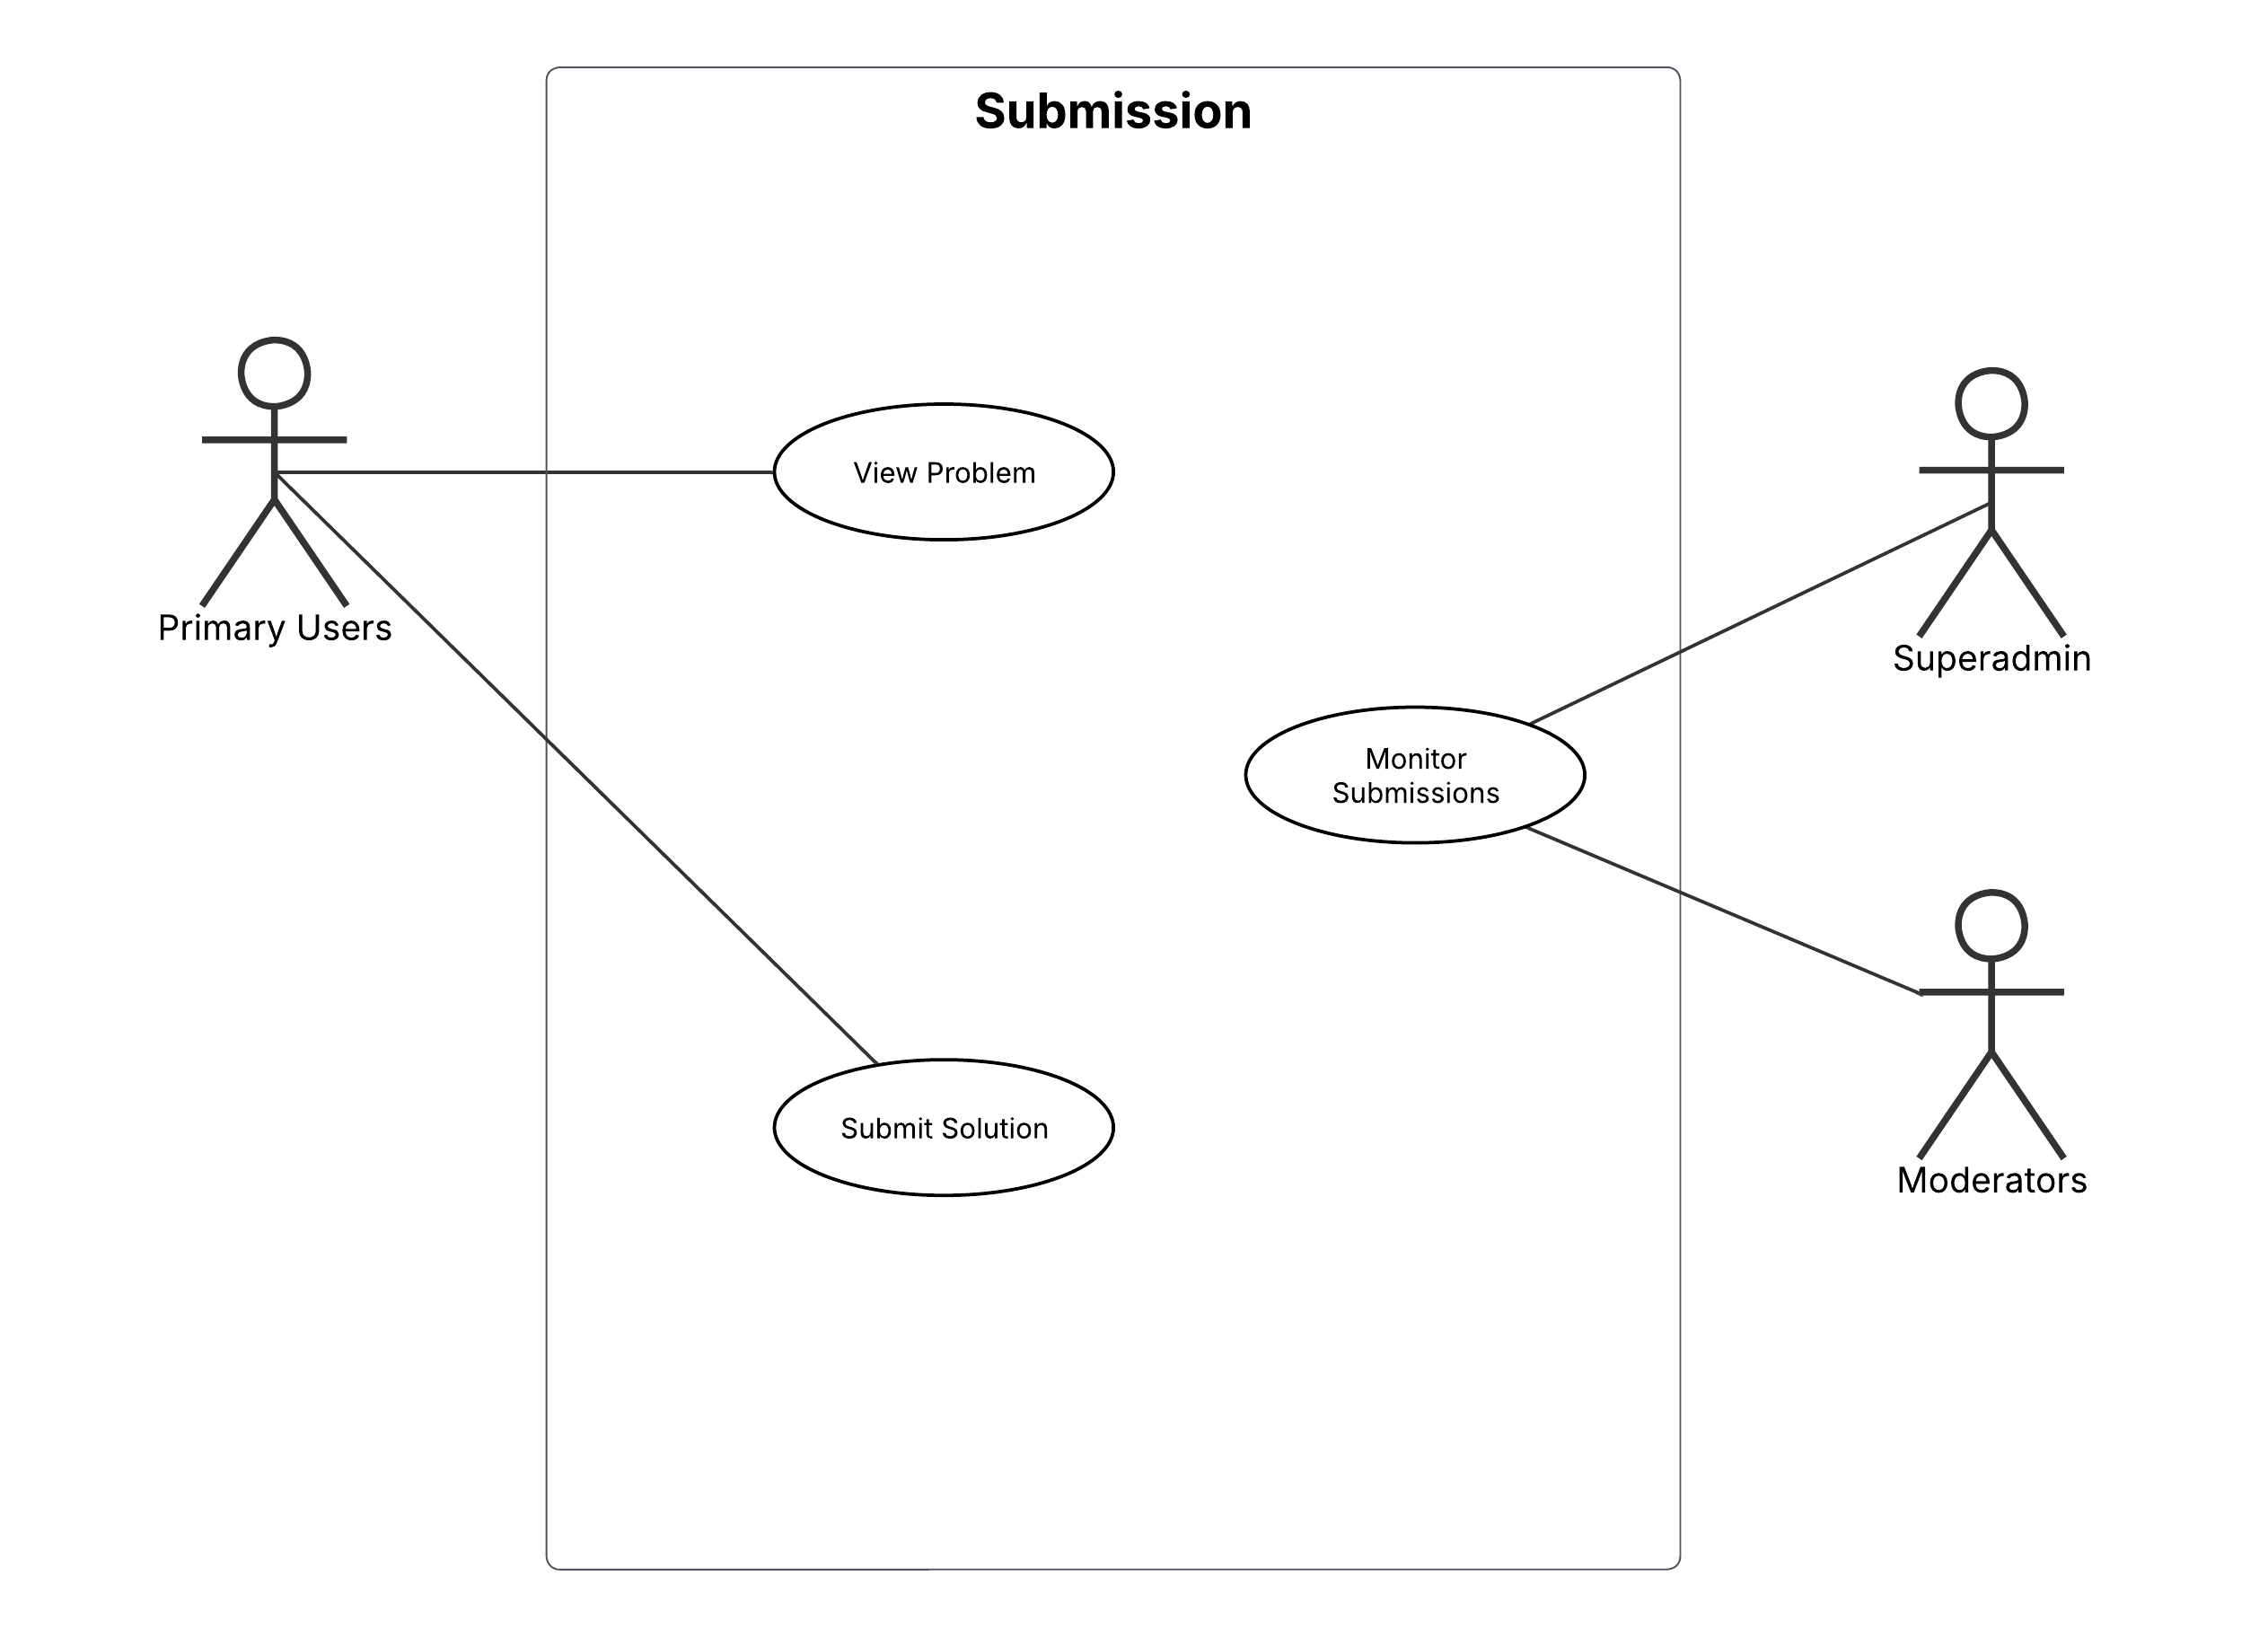
\includegraphics[width=1\textwidth]{Contents/Chapter 3/Usecase/Images/Submission.png}
    \vspace{0.6cm}
    \caption{Submission Use Case}
\end{figure}
The \textbf{Submission} submodule is the core execution engine and interaction point for all coding activities within the CodeRank system. Its primary function is to facilitate the practice and assessment workflow for the Primary User. Users begin by accessing the \textbf{View Problem} function, which presents the algorithmic challenge and requirements. The fundamental action in this module is the \textbf{Submit Solution} function, which securely receives the user's code, initiates the automatic grading process in a sandboxed environment, and returns the execution verdict. For oversight and quality assurance, both the Superadmin and Moderators are granted the ability to Monitor Submissions. This administrative function is vital for diagnosing issues with test cases, tracking potential cases of plagiarism, and ensuring the overall stability and fairness of the automated grading system.
\subsubsection{Use-case description tables}
% \begin{table}
% \caption{Use Case UC-1: Problems Management}
% \renewcommand{\arraystretch}{1.4}
% \begin{tabular}{|p{4cm}|p{11cm}|}
% \hline
% \textbf{ID and Name} & UC-1. Problems Management \\ \hline

% \textbf{Date Created} & 20th September, 2025 \\ \hline

% \textbf{Primary Actor} & Primary User, Superadmin, Moderator \\ \hline

% \textbf{Secondary Actor} & System (CodeRank Platform) \\ \hline

% \textbf{Description} &
% This use case describes how Moderators and Superadmins manage algorithmic problems on the platform. The process includes creating, editing, approving, and publishing problems. It also covers defining problem statements, input/output formats, constraints, sample test cases, and hidden test cases.
% \\ \hline

% \textbf{Trigger} &
% A Moderator or Superadmin decides to create, edit, approve, or publish a problem.
% \\ \hline

% \textbf{Preconditions} &
% \begin{itemize}
% \item The user is logged in as a Moderator or Superadmin.
% \item The problem management interface is accessible.
% \end{itemize}
% \\ \hline

% \textbf{Postconditions} &
% \begin{itemize}
% \item A new problem is created and saved as draft.
% \item A draft problem is updated or submitted for approval.
% \item A published problem may be updated after Superadmin approval.
% \item A problem is published once the approval rule is satisfied.
% \end{itemize}
% \\ \hline

% \textbf{Normal Flow} &
% \begin{enumerate}
% \item Moderator/Superadmin accesses the problem management interface.
% \item Moderator creates a new problem (saved as draft).
% \item Moderator edits draft problem (auto-saved).
% \item Moderator or Superadmin submits the problem for approval.
% \item Moderator approves problem → System checks publishing rule.
% \item If approvals >= 3 (Moderators) or 1 (Superadmin), system auto-publishes.
% \item Superadmin can directly approve and publish a problem.
% \end{enumerate}
% \\ \hline

% \textbf{Alternative Flow} &

% \textbf{AF–1:} Moderator edits a published problem → System saves changes as pending\_edit → Requires Superadmin approval. 

% \textbf{AF–2:} If approval threshold is not met, the problem stays pending until more approvals are collected.
% \\ \hline

% \textbf{Exceptions} &
% \textbf{E–1:} Superadmin rejects a pending edit → System notifies Moderator.
% \\ \hline
% \end{tabular}
% \end{table}


% \begin{table}
% \caption{Use Case UC-2: Contest Management}
% \renewcommand{\arraystretch}{1.3}
% \begin{tabular}{|p{4cm}|p{11cm}|}
% \hline
% \textbf{ID and Name} & UC-2. Contest Management \\ \hline

% \textbf{Date Created} & 20th September, 2025 \\ \hline

% \textbf{Primary Actor} & Primary User, Superadmin, Moderator \\ \hline

% \textbf{Secondary Actor} & System (CodeRank Platform) \\ \hline

% \textbf{Description} &
% This use case describes how users create and submit contests, allow administrators to review and approve them, and make contests available for participation once published.
% \\ \hline

% \textbf{Trigger} &
% A Primary User submits a new contest request.
% \\ \hline

% \textbf{Preconditions} &
% \begin{itemize}[nosep, leftmargin=*]
% \item The user is authenticated.
% \item Contest details (title, description, rules, problems) are provided.
% \item The contest submission form is valid.
% \end{itemize}
% \\ \hline

% \textbf{Postconditions} &
% \begin{itemize}[nosep, leftmargin=*]
% \item Contest status is updated (pending, approved, or published).
% \item Notifications are sent to users and admins.
% \item Users can participate in contests once published.
% \end{itemize}
% \\ \hline

% \textbf{Normal Flow} &
% \begin{enumerate}[nosep, leftmargin=*]
% \item Primary User submits a contest request.
% \item The System saves the contest as \textit{Pending Review}.
% \item Moderators review and approve the contest.
% \item If at least 3 moderator approvals are received, the contest qualifies for publishing.
% \item Alternatively, a Superadmin may approve and publish with a single approval.
% \item The System updates the contest status to \textbf{Published}.
% \item Notifications are sent to the contest creator and relevant moderators.
% \item Primary Users may now participate in the contest.
% \end{enumerate}
% \\ \hline

% \textbf{Alternative Flow} &
% \begin{itemize}[nosep, leftmargin=*]
% \item \textbf{AF-1: Insufficient Approvals}: If fewer than 3 moderator approvals are received, the contest remains in \textit{Pending Review}.
% \item \textbf{AF-2: Superadmin Override}: A Superadmin may publish directly, bypassing moderator approvals.
% \item \textbf{AF-3: Invalid Submission}: If contest data is incomplete or invalid, the submission is rejected with an error message.
% \end{itemize}
% \\ \hline

% \textbf{Exceptions} &
% \begin{itemize}[nosep, leftmargin=*]
% \item \textbf{E-1}: Database error when saving or updating the contest request.
% \item \textbf{E-2}: Approval action references a contest that does not exist.
% \item \textbf{E-3}: Notification delivery fails (system logs error, but contest status remains updated).
% \end{itemize}
% \\ \hline

% \end{tabular}
% \end{table}

% \begin{table}

% \renewcommand{\arraystretch}{1.3}
% \begin{tabular}{|p{4cm}|p{11cm}|}
% \caption{Use Case UC-3: Create a Discussion}
% \hline
% \textbf{ID and Name} & UC-3. Create a Discussion \\ \hline

% \textbf{Date Created} & 20th September, 2025 \\ \hline

% \textbf{Primary Actor} & Primary User \\ \hline

% \textbf{Secondary Actor} & System (CodeRank Platform) \\ \hline

% \textbf{Description} &
% This use case describes how a \textbf{Primary User} initiates a new discussion thread, typically linked to a specific problem ID or a general topic, setting the initial content and title.
% \\ \hline

% \textbf{Trigger} &
% The Primary User navigates to a problem page or the main forum and selects the \textit{"New Discussion"} option.
% \\ \hline

% \textbf{Preconditions} &
% \begin{itemize}[nosep, leftmargin=*]
% \item The user is authenticated.
% \item The discussion creation interface is accessible.
% \end{itemize}
% \\ \hline

% \textbf{Postconditions} &
% \begin{itemize}[nosep, leftmargin=*]
% \item A new discussion thread is created with the status \textit{"Active."}
% \item The discussion is visible to other Primary Users.
% \end{itemize}
% \\ \hline

% \textbf{Normal Flow} &
% \begin{enumerate}[nosep, leftmargin=*]
% \item Primary User accesses the problem/forum page and initiates creation.
% \item The user enters the discussion title and body content.
% \item The user submits the discussion.
% \item The system saves the new thread, assigns a unique ID, and displays it.
% \end{enumerate}
% \\ \hline

% \textbf{Alternative Flow} &
% \begin{itemize}[nosep, leftmargin=*]
% \item \textbf{AF-1: Content Validation Error}: If the title or body content is empty, the System displays an error message and requires the User to correct the input before submission.
% \end{itemize}
% \\ \hline

% \textbf{Exceptions} &
% \begin{itemize}[nosep, leftmargin=*]
% \item \textbf{E-1: Submission Failure}: If the database connection fails, the System displays a technical error and saves the content as a temporary draft (if possible).
% \end{itemize}
% \\ \hline

% \end{tabular}
% \end{table}

% \newpage

% \begin{table}[h!]
% \renewcommand{\arraystretch}{1.3}
% \begin{tabular}{|p{4cm}|p{11cm}|}
% \caption{Use Case UC-4: Submit a Solution}
% \hline
% \textbf{ID and Name} & UC-4. Submit a Solution \\ \hline

% \textbf{Date Created} & 20th September, 2025 \\ \hline

% \textbf{Primary Actor} & Primary User \\ \hline

% \textbf{Secondary Actor} & System (CodeRank Platform), Worker Service \\ \hline

% \textbf{Description} &
% This use case describes the primary mechanism for a \textbf{Primary User} to select a programming language, submit their solution code for a problem they are currently viewing, and receive an automated verdict on its correctness and efficiency.
% \\ \hline

% \textbf{Trigger} &
% The Primary User clicks the \textit{"Submit"} button on a coding problem interface after entering or selecting their solution code.
% \\ \hline

% \textbf{Preconditions} &
% \begin{itemize}[nosep, leftmargin=*]
% \item The user is authenticated.
% \item The user is currently viewing an active problem.
% \item The user has selected a supported programming language.
% \item The code is syntactically valid (pre-checked client-side).
% \end{itemize}
% \\ \hline

% \textbf{Postconditions} &
% \begin{itemize}[nosep, leftmargin=*]
% \item The submitted code is sent to the System.
% \item The Submission History is updated with the result (e.g., Accepted, Wrong Answer).
% \item The user's score and statistics are updated based on the verdict.
% \end{itemize}
% \\ \hline

% \textbf{Normal Flow} &
% \begin{enumerate}[nosep, leftmargin=*]
% \item Primary User is on the problem page and selects their preferred language.
% \item The user enters or pastes the solution code into the editor.
% \item The user clicks \textit{"Submit."}
% \item The system validates the submission (e.g., code length, language availability).
% \item The system sends the code and the problem's hidden test cases to the Worker Service.
% \item \textbf{Worker Service} securely executes the code and determines the verdict (e.g., Accepted, Time Limit Exceeded, Runtime Error).
% \item The system displays the final verdict and execution statistics to the Primary User.
% \end{enumerate}
% \\ \hline

% \textbf{Alternative Flow} &
% \begin{itemize}[nosep, leftmargin=*]
% \item \textbf{AF-1: Attempted Language Not Supported}:  
% If the user attempts to submit code in a language that is not currently enabled for the problem, the System displays an error and requires the user to change their language selection.
% \end{itemize}
% \\ \hline

% \textbf{Exceptions} &
% \begin{itemize}[nosep, leftmargin=*]
% \item \textbf{E-1: Submission Failure}:  
% If the sandbox environment or the external grading service fails during execution, the System logs the error and returns a \textit{"System Error"} verdict to the user, advising them to try again later.
% \end{itemize}
% \\ \hline

% \end{tabular}
% \end{table}


\newpage

\section{Architecture Diagram}
\subsection{Architectural Decision Rationale}
Architectural diagrams provide a structured view of how a software system is organized and how its components interact. In modern software development, two primary architectural styles are commonly considered: \textbf{monolithic architecture} and \textbf{microservice architecture}.

A \textbf{monolithic architecture} is a traditional model of a software program, which is built as a unified unit that is self-contained and independent from other applications. The word “monolith” is often attributed to something large and glacial, which isn’t far from the truth of a monolith architecture for software design. \cite{atlassian_microservices_vs_monolith}

A \textbf{microservices architecture}, also simply known as microservices, is an architectural method that relies on a series of independently deployable services. These services have their own business logic and database with a specific goal. Updating, testing, deployment, and scaling occur within each service. Microservices decouple major business, domain-specific concerns into separate, independent code bases. \cite{atlassian_microservices_vs_monolith}

As can be seen, the choice between these architectural approaches depends on the project’s specific requirements, team size, and long-term goals. Smaller systems or teams often benefit from the straightforwardness of monolithic architecture, while larger, more complex systems may require the flexibility and scalability of distributed services.

After evaluating our project goals and team size, we decided to implement a service-based modular monolith as the core architectural foundation for CodeRank. The key reasons for selecting this approach include:
\begin{itemize}
    \item \textbf{Team Size and Feasibility}
With only two members, adopting a full microservice architecture would introduce significant overhead in DevOps, deployment, and service management. In contrast, a modular monolith allows us to focus on implementing core features without the burden of distributed complexity.
    \item \textbf{Easier Development and Maintenance}
By separating the system into modules—such as the Discussion Module, Submission Module, Auth Module, and Contest Module—we can maintain clean boundaries within a single codebase. This structure enables faster development cycles and reduces merging conflicts.
    \item \textbf{Future Scalability}
While CodeRank currently operates as a monolithic application, its modules are designed following \textbf{Domain-Driven Design} (DDD) principles. These boundaries can later be extracted into microservices if the system needs to scale. This ensures long-term flexibility without requiring microservices prematurely.
\end{itemize}
\begin{figure}[h!]
    \centering
    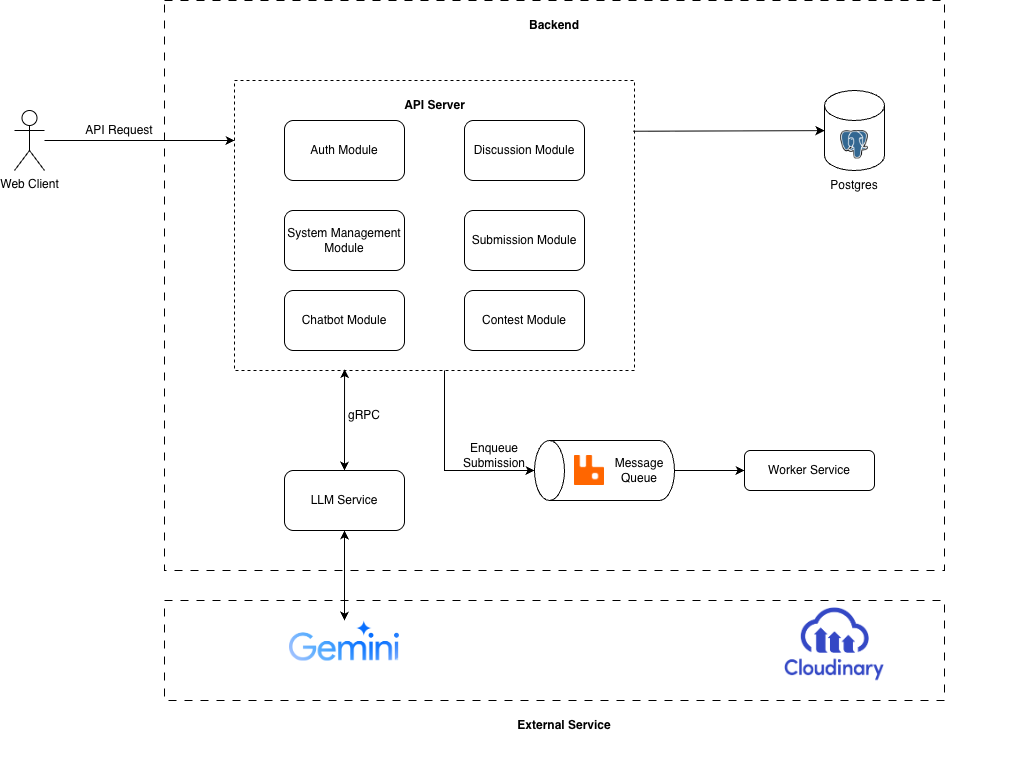
\includegraphics[width=1\textwidth]{Contents/Chapter 3/Architecture Diagram/CodeRank.drawio.png}
    \vspace{0.6cm}
    \caption{Architecture Diagram}
    \label{fig:leetcode-system}
\end{figure}
\clearpage

\subsection{System Components}

\begin{figure}[h!]
    \centering
    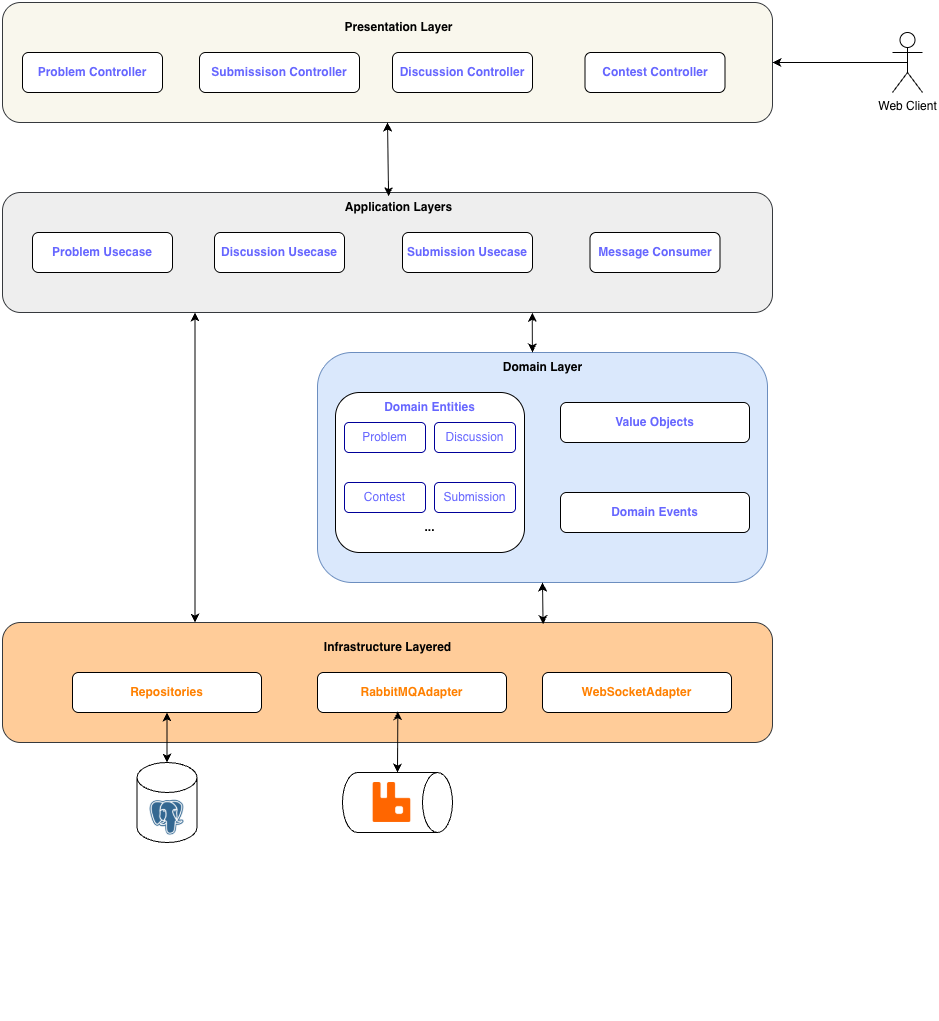
\includegraphics[width=1\textwidth]{Contents/Chapter 3/Architecture Diagram/LayeredArchitecture.drawio.png}
    \vspace{0.6cm}
    \caption{Layered Architecture}
    \label{fig:leetcode-system}
\end{figure}
The system architecture of CodeRank is organized into four primary layers, each responsible for a specific set of functions. This layered approach ensures clean separation of concerns, maintainability, and a clear mapping between business rules and system implementation.

\begin{enumerate}
  \item \textbf{Presentation Layer}
  
The \textbf{Presentation Layer} acts as the entry point for all external interactions with the system. It exposes various controllers such as the \textit{Problem Controller}, \textit{Submission Controller}, \textit{Discussion Controller}, and \textit{Contest Controller}, which handle incoming HTTP requests from the web client. These controllers validate user input, map requests to the appropriate application use cases, and return responses in a structured format. This layer focuses purely on communication and does not contain business logic, ensuring the interface remains thin and easily adaptable.
    \item  \textbf{Application Layer}
    
The \textbf{Application Layer} contains the system’s core orchestrators, known as Use Cases. Examples include the Problem Usecase, Discussion Usecase, Submission Usecase, and a dedicated Message Consumer for asynchronous tasks.

This layer coordinates operations between the Presentation Layer and the Domain Layer, ensuring that business rules are executed in the correct sequence. It does not implement business rules itself; instead, it acts as a mediator, invoking domain logic and triggering events. This design improves code clarity and supports future expansion.

    \item  \textbf{Domain Layer}
    
The \textbf{Domain Layer} represents the heart of the application, where all business logic and system rules are defined. It contains: 

\begin{itemize}
    \item Domain Entities such as Problem, Discussion, Contest, and Submission.
    \item Value Objects that encapsulate immutable attributes or concepts.
Domain Events used to capture and react to significant changes within the system.
    \item Domain Events used to capture and react to significant changes within the system.
\end{itemize}

    \item  \textbf{Infrastructure Layer}
    
The \textbf{Infrastructure Layer} provides the technical capabilities required to support the domain and application layers. It includes: 

\begin{itemize}
    \item \textbf{Repositories}, which manage communication with the PostgreSQL database.
    \item \textbf{RabbitMQ Adapters}, responsible for publishing and consuming messages for asynchronous processing.
Domain Events used to capture and react to significant changes within the system.
    \item \textbf{WebSocket Adapters}, enabling real-time communication such as live updates for submissions or discussion activities.
\end{itemize}

This layer abstracts external systems and framework-specific operations, ensuring that the upper layers remain decoupled from technical implementation details.

\end{enumerate}
\section{Code Runner}
\subsection{Overview}
\textbf{Code Runner} Component is a core component of Submission Worker Service, responsible for executing user-submitted programs against predefined test cases. It serves as a bridge between the user’s solution and the problem’s input–output data, ensuring fair and consistent evaluation. 
For each programming language supported by the platform (C++, Java, Python), a specific implementation of the \textbf{Code Runner} will be developed to handle language-specific compilation, execution, and output parsing. This ensures that user code is run correctly and consistently, regardless of the language chosen.
\subsection{Class Diagram}
\begin{figure}[h!]
    \centering
    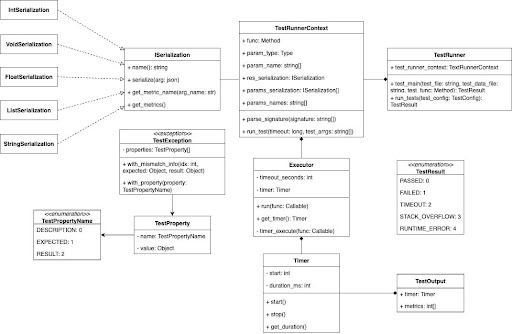
\includegraphics[width=1\textwidth]{Contents/Chapter 3/Code Runner/CodeRunner.jpg}
    \vspace{0.6cm}
    \caption{Class Diagram for Code Runner}
    \label{fig:leetcode-system}
\end{figure}

\begin{itemize}
    \item \textbf{ISerialization \& Implementations}: ISerialization defines a common interface for converting data between raw test inputs/outputs and program variables. Its implementations — IntSerialization, FloatSerialization, StringSerialization, ListSerialization, and VoidSerialization — handle serialization for different data types, ensuring test cases are interpreted correctly regardless of format.
    \item \textbf{TestRunnerContext}: TestRunnerContext stores the configuration and metadata needed to execute a user’s function, including parameter types, serializers, and the function reference itself. It prepares the environment for test execution and delegates the actual running to the Executor.
    \item \textbf{Executor}: Executor manages controlled execution of user-submitted functions. It enforces time limits, measures execution duration using Timer, and handles potential runtime issues like timeouts or errors during function calls.
    \item \textbf{Timer}: Timer measures how long each test case takes to execute. It provides simple start, stop, and duration tracking methods to record performance metrics for user solutions.
    \item \textbf{TestOutput}: TestOutput captures the results of a single test execution, storing both the runtime duration and any performance metrics. It is used to report how efficiently and accurately a user’s code performed.
    \item \textbf{TestException}: TestException represents errors or mismatches that occur during test execution. It stores details such as expected versus actual results and additional context through TestProperty objects.
    \item \textbf{TestProperty \& TestPropertyName}: TestProperty stores metadata about a test, such as a description or result comparison, identified by a TestPropertyName enum. These properties provide structured details for debugging failed test cases.
    \item \textbf{TestRunner}: TestRunner is the main controller responsible for running user code against predefined test cases. It coordinates between the TestRunnerContext, Executor, and ISerialization system to execute tests and produce final TestResult outcomes.
    \item \textbf{Solution}: Solution is the submission for the problem from the user.
\end{itemize}
\subsection{Testcase Format}
Each problem in the Online Judging System is accompanied by a test case file, named \textit{problem\_slug.csv}. This file defines a structured list of input–output test pairs used by the Test Runner of Worker Service to evaluate user submissions automatically.Moderators or superadmin upload this file when creating or updating a problem. The judging system parses the CSV, runs user code against each test case, and compares the output with the expected result.

To ensure accurate and consistent evaluation of user submissions, each input and output value in the \textit{problem\_slug.csv}file is associated with a data type. The type system defines how each field should be parsed, validated, and compared during the judging process.This mechanism helps the Test Framework interpret user program outputs correctly, whether they are numbers, strings, booleans, or lists. The following table describes the type.Here is the content for the "Problem Storages" section, including the table about type format:

\begin{table}[h!]
\centering
\renewcommand{\arraystretch}{1.3}
\begin{tabular}{|p{4cm}|p{10cm}|}
\hline
\textbf{Type Token} & \textbf{Description} \\ \hline

int & Integer numbers. \\ \hline

float & Floating-point numbers. \\ \hline

boolean & Boolean data. \\ \hline

string & Textual data. \\ \hline

void & Represents the absence of a value (e.g., for functions that return nothing). \\ \hline

list(type) & A collection of elements of a specified type (e.g., list(int)). \\ \hline

\end{tabular}
\caption{Data Types for Testcase Fields}
\end{table}
Each problem’s test case file will contain both type definitions for input, expected output and test data. The first line of the file specifies the data types for all inputs and outputs, helping the Test Runner correctly parse and validate values before running tests.

After executing all test cases for a user’s submission, the Test Runner generates a structured JSON result file summarizing the outcomes of each test. This file serves as the standardized output for the judging system and can be used by other services (such as the Result Service or API Gateway) to record, display, or analyze user performance. The JSON format ensures that results are machine-readable, language-independent, and easy to integrate into the overall online judging pipeline. The exported JSON file contains both metadata (e.g., problem name, language, execution status) and detailed per-test results (e.g., input, output, expected result, duration, and status).

\section{Ranking System}

The ranking system is a core component of the platform, designed to motivate users, reflect individual learning progress, and encourage healthy competition among participants. It provides a transparent and consistent mechanism for evaluating user performance based on problem-solving activities.

\subsection*{Overall Ranking Mechanism}

The platform maintains a global leaderboard that ranks all registered users based on their accumulated points obtained from solving programming problems. This leaderboard reflects the relative standing of users across the entire system and allows learners to compare their progress with others. However, to reduce server workload and avoid unnecessary real-time synchronization, the ranking data is not pushed to clients in real time.

Instead, the frontend retrieves ranking data through the backend API when users access or refresh the leaderboard page. The backend calculates or returns the latest available ranking data based on accepted submissions and accumulated user scores. This request-based approach keeps the implementation simple and efficient while still providing users with sufficiently updated ranking information during normal platform usage.

Although the leaderboard is not updated through real-time events, users can view their current score and ranking information whenever the relevant page or profile data is loaded from the backend. This design provides a practical balance between system performance, implementation complexity, and user experience.

\subsection*{Point Allocation per Problem}

Points are awarded based on the difficulty level of each problem. The platform categorizes problems into three difficulty levels, each associated with a predefined base score:
\begin{itemize}
    \item \textbf{Easy}: 100 points
    \item \textbf{Medium}: 150 points
    \item \textbf{Hard}: 200 points
\end{itemize}

This scoring scheme encourages users to challenge themselves with more complex problems while still recognizing achievements at all difficulty levels.

\subsection*{Penalty for Failed Submissions}

To promote code quality and thoughtful problem-solving, the system applies a penalty for unsuccessful submissions. A submission is considered failed if it does not pass all predefined test cases. For each failed submission attempt, a penalty of 10 points is deducted from the base score of the corresponding problem.

If the total penalty incurred from failed submissions exceeds the base score of the problem, the final score awarded for that problem is capped at 0 points. Negative scores are not applied. This mechanism discourages excessive trial-and-error submissions while still allowing users to continue practicing without additional penalties once the minimum score is reached.

\subsection*{First Successful Submission Policy}

Points are awarded only for the first successful submission of a problem, defined as the first submission that passes all test cases. Any subsequent successful submissions for the same problem are treated strictly as practice attempts and do not contribute additional points to the user’s total score.

This policy ensures fairness in the ranking system and prevents users from inflating their scores by repeatedly submitting solutions to the same problem. It also emphasizes learning progression through solving new problems rather than optimizing repeated submissions for ranking purposes.

\section{Database Design}

For data models design, we utilize Entity–Relationship Diagram (ERD) to capture the conceptual model of CodeRank System. It visualizes the core entities of the platform—such as users, problems, submissions, test cases, and judging results—and the relationships among them. The ERD serves a similar purpose to a UML class diagram, but at a higher level of abstraction. Therefore, including both diagrams would be redundant, and the ERD alone is sufficient for representing the system’s conceptual data structure.

The conceptual data model includes the following entities that will be grouped according to its business in our system. However, this diagram does not include all attributes of each entity for simplicity of illustration, but the essential ones are mentioned in the descriptions below.

\begin{figure}[H]
    \centering
    \rotatebox{90}{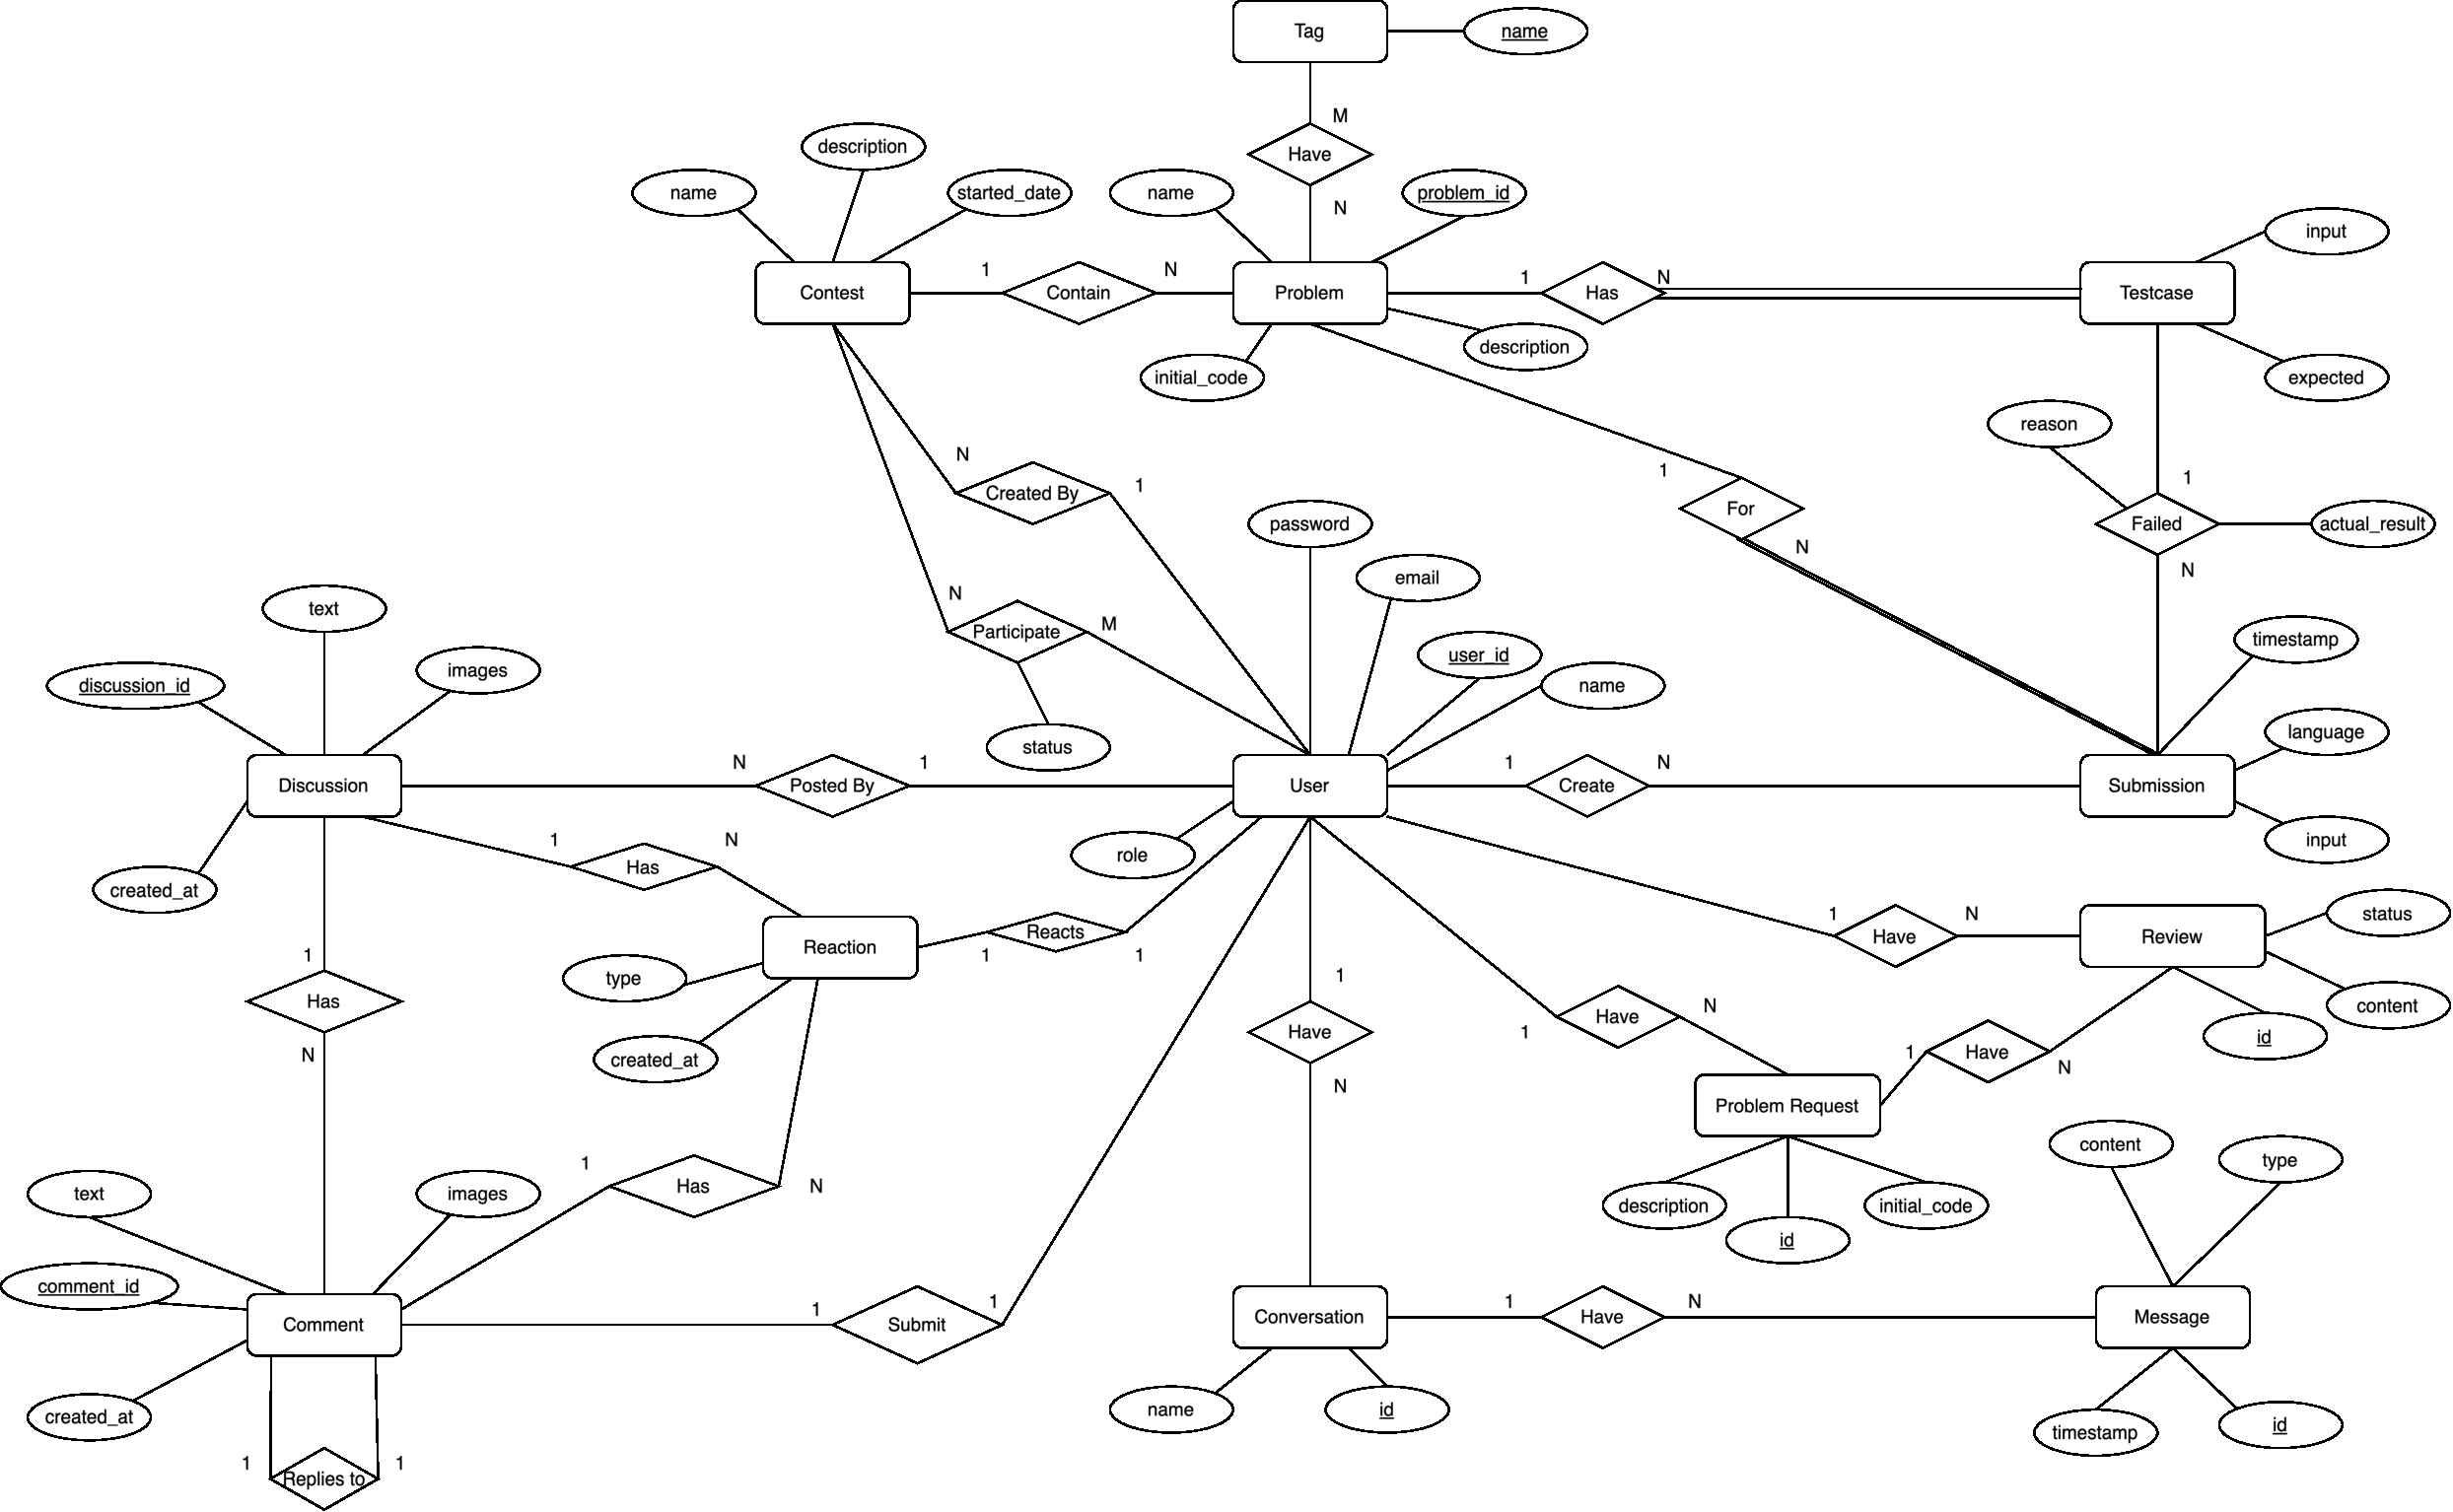
\includegraphics[width=\textheight]{Contents/Chapter 3/Database Design/erd.pdf}}
    \caption{Entity Relationship Diagram}
\end{figure}

\subsection*{User}
\begin{itemize}
    \item \textbf{User}: This abstract entity represents a user of the CodeRank system, storing essential information such as username, email, password hash. Each entity is identified by \textit{user\_id} For simplicity of illustration, we have omitter user roles and permissions in the ERD, all of this is represented by the attribute \textit{role} of the User entity. However, in the actual implementation, user roles and permissions will be managed through Role-Based Access Control (RBAC) to ensure secure and appropriate access to system functionalities.
\end{itemize}

\subsection*{Problems Solving}

\begin{itemize}
    \item \textbf{Problem}: Represents an algorithmic challenge that users can attempt to solve. Each problem includes a unique identifier \textit{problem\_id}, a title, a textual description, and optional starter code (\textit{initial\_code}) to guide users.
A problem may belong to multiple contests and can have multiple tags for classification.
    \item \textbf{Tag}: The \textit{Tag} entity helps organize problems into conceptual groups (for example, Dynamic Programming, String, etc). Each tag has a \textit{name} and may be associated with multiple problems through a many-to-many relationship.
    \item \textbf{Testcase}: Belongs to one problem and includes input data and the corresponding expected output. Testcases are used during code execution to validate user submissions.
    \item \textbf{Submission}: Represents a user's attempt to solve a problem. Each submission is linked to a specific user and problem, and includes the submitted code, programming language, timestamp, and status (e.g., pending, accepted, rejected).
\end{itemize}

\subsubsection*{Problems Management}

\begin{itemize}
    \item \textbf{Problem Request}: Represents a request made by a moderator or superadmin to add a new problem to the platform. Each request includes a title, description, and status (e.g., pending, approved, rejected). It is linked to the moderator or superadmin who made the request.
    \item \textbf{Review}: Represents the review process for a problem request. Each review is associated with a specific problem request and includes feedback, status (e.g., approved, rejected), and the timestamp of the review. It is linked to the moderator or superadmin who conducted the review.
\end{itemize}

\subsection*{Contest}
\begin{itemize}
    \item \textbf{Contest}: Represents a coding competition that users can participate in. Each contest includes a unique identifier \textit{contest\_id}, a title, description, start time, end time, and a list of problems included in the contest. A contest will contain many problems, anc can have many participants.
\end{itemize}

\subsection*{Interview Practice}

\begin{itemize}
    \item \textbf{Conversation}: Represents a coding interview session between a Primary User and chatbot system. Each conversation includes a unique identifier \textit{conversation\_id}, start time, end time. Each conversation is linked to the Primary User who initiated it.
    \item \textbf{Message}: Represents individual messages exchanged during a coding interview conversation. Each message includes a unique identifier \textit{message\_id}, timestamp, content, and type of the message. If the message comes from Primary User, the type will be \textit{user}, otherwise \textit{system}. Each message is linked to the conversation it belongs to.
\end{itemize}

\subsubsection*{Discussion}
\begin{itemize}
    \item \textbf{Discussion}: represents forum-like discussion threads associated with a topic. Users can post questions, explanations, optimization ideas, or clarifications. Each discussion entry may contain text and optional images, and it records creation timestamps.
    \item \textbf{Comment}: Users can comment on discussion threads, forming a threaded conversation system. Each comment includes text, optional images, and a timestamp.
    \item \textbf{Reaction}: Users can react to both discussions and comments using predefined reaction types (e.g., like, love, insightful). Each reaction records the type of reaction and the user who made it.
\end{itemize}

To summarize the relationships among these entities:
\begin{itemize}
    \item A \textbf{User} can \textbf{submit} multiple \textbf{Submission}.
    \item Each \textbf{Submission} is \textbf{linked} to one \textbf{User} and one \textbf{Problem}.
    \item A \textbf{Problem} can \textbf{have} multiple \textbf{Testcases} and can be \textbf{associated} with multiple \textbf{Tags}.
    \item A \textbf{Contest} can \textbf{have} multiple \textbf{Users} as participants.
    \item A \textbf{Contest} can \textbf{include} multiple \textbf{Problem}.
    \item A \textbf{Problem Request} is made by a \textbf{User} with moderator or superadmin role.
    \item A \textbf{Review} is \textbf{conducted} by a \textbf{User} with moderator or superadmin role for a specific \textbf{Problem Request}.
    \item A \textbf{Conversation} is \textbf{initiated} by a \textbf{User} with Primary role.
    \item A \textbf{Conversation} can have multiple \textbf{Messages}.
    \item A \textbf{Discussion} can have multiple \textbf{Comments} and \textbf{Reactions}, and each \textbf{Comment} can also have multiple \textbf{Reactions}.
    \item A \textbf{Tag} can be associated with multiple \textbf{Problems}.
\end{itemize}


\section{Chatbot Design}
\subsection{Overview}
A chatbot, short for "chat robot", is an artificial intelligence (AI) software designed to simulate conversations with human users, especially over the internet. They interact with humans in their natural languages, typically through messaging applications, mobile apps or through a website. Chatbots can be programmed to respond the same way each time, to respond differently to messages containing specific keywords, or to use machine learning to adapt their responses to fit the situation. \cite{chatbot_definition}

In the context of CodeRank System, the chatbot is an AI-powered interactive interview coach designed to assist learners practicing technical coding interviews, particularly algorithm problems. The system leverages Google Gemini as the underlying large language model (LLM) and LangChain as the orchestration framework that structures prompts, manages conversational flow, and implements contextual memory.

The goal of the chatbot is to simulate real interview scenarios through step-by-step dialogue, enabling learners to experience guided practice, receive hints, refine answers, and develop a deeper understanding of algorithmic problem-solving techniques. To achieve human-like interaction, the chatbot must:
\begin{enumerate}
    \item Understand user inputs
    \item Maintain awareness of previous exchanges
    \item Adapt its questioning based on user responses
    \item Provide constructive and relevant feedback
    \item Prevent context loss during long interview sessions
\end{enumerate}

\subsection{Use case analysis}
To ensure consistent behavior and maintain the structured flow of a technical interview, the chatbot uses a System Prompt, also known as a behavioral instruction prompt. This prompt defines the chatbot's role as an AI interview coach and outlines the rules that govern how it interacts with the user. The following system prompt defines the chatbot's role and behavior during the structured mock interview process:
\begin{tcolorbox}[
    colback=white,      % White background
    colframe=black,     % Black border
    boxrule=0.8pt,      % Border thickness
    breakable,          % Allow page breaks
    sharp corners,      % Square corners
    listing only,       % Use listings engine
    listing options={
        basicstyle=\ttfamily\small,
        breaklines=true,      % Wrap long lines
        columns=fullflexible  % Prevent overflow
    }
]
\begin{verbatim}
You are an AI interview coach for coding interviews.
Your job is to conduct a structured mock interview.

Rules:
1. The FIRST message you receive from the user is the topic they want
to practice (e.g., arrays, dynamic programming, graphs).

2. After the user chooses a topic, ask ONE coding problem at a time.

3. After giving a question:
   - Wait for the user’s solution attempt.
   - Do NOT evaluate until the user submits a solution.
   - If the user is not ready, ask them to type their solution 
   when ready.

4. Provide hints ONLY when:
   - The user explicitly asks for a hint, OR
   - The user gives 3 incorrect attempts.

5. After the user solves (or gives up), provide:
   - A concise explanation
   - Optimal solution
   - Time complexity
   - Space complexity

6. Stay in interview mode.
\end{verbatim}
\end{tcolorbox}

To support a smooth and structured technical interview experience, the chatbot must be able to recognize different categories of user intentions. For the interview practice module of the CodeRank System, we classify user intents into three primary types: topic selection, problem-solving intent, and hint-seeking behavior. Each intent triggers a specific dialogue pattern that aligns with the structured mock interview workflow.

\textbf{Topic Selection Intent:} When users explicitly mention an interview topic, 
such as arrays, graphs, or dynamic programming, the system interprets this as an 
intention to begin or switch an interview topic. The chatbot should confirm the 
topic and proceed to present an appropriate coding problem. The possible questions are “Let’s practice arrays.”, “I want to try a dynamic 
programming problem.”, “Graphs.”, ...

\textit{For example when the user wants to find a topic to practice:}

\begin{quote}
\textbf{User:} Find me an array problem.\\
\textbf{Chatbot:} Sure! We'll practice arrays. Here is your first problem: 
\textit{Given an integer array…} Please let me know when you're ready to 
provide your solution.
\end{quote}

If the user provides additional details, the chatbot refines the difficulty:

\begin{quote}
\textbf{User:} Give me an easy array problem.\\
\textbf{Chatbot:} Great! Here is an easy-level array problem for you…
\end{quote}

\textbf{Problem-Solving Intent:} Once a coding problem has been presented, the user may 
respond with a complete solution, partial reasoning, or follow-up questions. This indicates 
the intention to solve the problem. The chatbot should acknowledge the attempt, avoid 
evaluating prematurely, and respond only after the user explicitly submits their solution. Possible user messages include “Here is my solution…”, “Does this approach work?”, 
or “I think we can use two pointers.”

\textit{For example when the user wants to submit a solution:}

\begin{quote}
\textbf{User:} Here is my solution: \texttt{...code...}\\
\textbf{Chatbot:} Thanks! Let me review your solution.
\end{quote}

If the user is still thinking:

\begin{quote}
\textbf{User:} I'm not ready yet.\\
\textbf{Chatbot:} No problem—take your time. Let me know when you're ready to submit 
your solution.
\end{quote}

If the attempt is incorrect, the chatbot guides without revealing too much:

\begin{quote}
\textbf{Chatbot:} This is not fully correct. Try again—pay attention to the edge case 
where the array may contain duplicates.
\end{quote}

\textbf{Hint-Seeking Intent:} When the user explicitly asks for help or expresses that they 
are stuck, the system recognizes this as an intention to request a hint. According to the 
interview rules, hints should only be provided when requested or after three unsuccessful 
attempts. Possible user messages include “Give me a hint.”, “I’m stuck.”, or “Can you guide me?”

\textit{For example when the user requests assistance:}

\begin{quote}
\textbf{User:} I’m stuck. Give me a hint.\\
\textbf{Chatbot:} Sure! Here’s a hint: Try using a hash map to store the frequencies of 
elements before making your decision.
\end{quote}

If the user is unclear about what type of hint they need:

\begin{quote}
\textbf{User:} I need help.\\
\textbf{Chatbot:} Of course. Would you like a conceptual hint, or guidance on improving 
your current approach?
\end{quote}

\section{Chatbot Design}

This chapter presents the detailed architecture, design decisions, and implementation of the chatbot subsystem in the CodeRank system. The chatbot is designed as an AI-powered coding interview assistant capable of simulating real-world technical interview scenarios.

Unlike traditional rule-based chatbots, the proposed system leverages a large language model combined with a workflow orchestration layer to enable adaptive reasoning, contextual memory, and dynamic response generation. This allows the system to behave as an intelligent interviewer that can guide users through structured problem-solving processes.

\subsection{N8N Integration Architecture}

The chatbot subsystem is implemented on top of \textbf{n8n}, which acts as a central orchestration layer connecting the frontend interface, backend services, and the Gemini large language model.

Instead of establishing a direct communication channel between the frontend and the LLM provider, all chatbot requests are routed through n8n workflows. This architectural decision introduces a middleware layer responsible for handling request processing, prompt management, memory retrieval, and response generation logic.

By decoupling AI logic from application layers, the system achieves better separation of concerns and improves maintainability in large-scale development.

\textbf{System Benefits:}
\begin{itemize}
    \item \textbf{Separation of Concerns:} AI logic is isolated from frontend and backend business logic, reducing system coupling.
    
    \item \textbf{Centralized Workflow Management:} All chatbot-related logic is managed in a single workflow system, making it easier to modify prompts, behaviors, and processing rules.
    
    \item \textbf{Improved Maintainability:} Changes in AI behavior do not require modifications in frontend or backend codebases.
    
    \item \textbf{Observability:} n8n provides execution logs at each node level, enabling easier debugging and monitoring of AI interactions.
\end{itemize}

\textbf{Chatbot Communication Flow:}
\begin{enumerate}
    \item The user interacts with the chatbot through the CodeRank frontend interface.
    
    \item The frontend sends the user message along with metadata to a backend API endpoint.
    
    \item The backend validates the request and triggers an n8n workflow via a webhook.
    
    \item The n8n workflow processes the request through a series of structured nodes.
    
    \item The workflow communicates with the Gemini model to generate context-aware responses.
    
    \item The final response is returned through the backend API and rendered in the frontend interface.
\end{enumerate}

This layered architecture enables independent evolution of system components, allowing AI logic, backend services, and frontend interfaces to be updated without affecting each other significantly.

\subsection{AI Agent Workflow Design in n8n}

The chatbot workflow is designed as an AI agent pipeline that simulates structured human-like reasoning during technical interview sessions. The workflow is composed of multiple modular stages, where each stage is responsible for a specific transformation or processing step.

This design follows a pipeline-based architecture, ensuring that input processing, context management, reasoning, and output generation are clearly separated.

\textbf{Workflow Stages:}
\begin{enumerate}
    \item User input reception
    \item Context and memory retrieval
    \item Prompt construction
    \item LLM processing
    \item Response post-processing
    \item Response delivery
\end{enumerate}

Each stage plays a critical role in ensuring that the chatbot maintains coherence, contextual awareness, and domain-specific behavior during long interview sessions.

\subsubsection{Webhook Trigger}

The workflow begins with a \textbf{Webhook Trigger Node}, which serves as the entry point for all incoming chatbot requests.

This node receives HTTP requests from the backend containing structured data such as:
\begin{itemize}
    \item User message content
    \item Conversation identifier for session tracking
    \item Interview context or selected topic
    \item User-related metadata (e.g., difficulty level, session state)
\end{itemize}

The webhook ensures that every interaction is properly initialized within the workflow execution context, enabling traceability and session continuity.

\subsubsection{Context and Memory Management}

One of the key challenges in conversational AI systems is maintaining context across multiple turns of interaction. To address this, the system implements a memory management mechanism within the workflow.

Before generating a response, the system retrieves relevant historical data including:
\begin{itemize}
    \item Previously asked interview questions
    \item User-submitted solutions or attempts
    \item Feedback and hints provided by the system
    \item Current interview progression state
\end{itemize}

This memory mechanism allows the chatbot to maintain consistency across long sessions and avoid treating each message as an isolated input. As a result, the AI behaves more like a continuous interviewer rather than a stateless response generator.

\subsubsection{Prompt Construction}

After retrieving contextual information, the system constructs a structured prompt that will be sent to the large language model.

The prompt construction process combines multiple sources of information:
\begin{itemize}
    \item System-level instructions defining chatbot behavior
    \item Current user input message
    \item Conversation history retrieved from memory
    \item Interview state and difficulty configuration
\end{itemize}

This step is crucial because prompt quality directly impacts the performance and consistency of the LLM output. By explicitly structuring the prompt, the system ensures that Gemini follows the expected interview logic and generates responses aligned with the CodeRank learning objectives.

\subsubsection{LLM Processing with Gemini}

The constructed prompt is passed to the \textbf{Google Gemini Chat Model node} within n8n. This node is responsible for interacting with the Gemini API and generating the final response based on the provided context.

The Gemini model performs multiple reasoning tasks simultaneously, including:
\begin{itemize}
    \item Understanding user intent in a programming context
    \item Generating coding interview questions dynamically
    \item Providing step-by-step hints for problem-solving
    \item Evaluating user approaches and suggesting optimizations
\end{itemize}

Depending on the state of the conversation, the model can act as an interviewer, tutor, or evaluator, allowing flexible adaptation to different learning scenarios.

\subsubsection{Response Post-processing}

After receiving the output from the LLM, the system performs a post-processing stage to ensure that the response is suitable for frontend rendering.

This includes:
\begin{itemize}
    \item Formatting output into Markdown-compatible structure
    \item Removing unnecessary tokens or artifacts
    \item Validating response completeness and structure
    \item Logging interaction data for debugging and analytics
\end{itemize}

This step ensures that the final response is clean, consistent, and user-friendly when displayed in the chatbot interface.

\subsubsection{Frontend Delivery}

The final processed response is returned through the backend API to the frontend application. The frontend then renders the response in real time within the chat interface.

This completes the full request-response cycle, enabling an interactive and low-latency conversational experience for users during coding interview sessions.

\subsection{System Design Benefits}

The proposed chatbot architecture provides several important system-level advantages:

\begin{itemize}
    \item \textbf{Modular Architecture:} Each stage of the workflow is independently defined, allowing easy modification and extension without affecting the entire system.
    
    \item \textbf{Scalability:} The system can be extended to support additional AI features such as retrieval-augmented generation (RAG), multi-agent collaboration, or external knowledge integration.
    
    \item \textbf{Maintainability:} Centralized workflow logic reduces code duplication and simplifies long-term maintenance.
    
    \item \textbf{Flexibility:} New AI behaviors can be introduced by modifying workflow nodes without changing core application code.
    
    \item \textbf{Observability:} Built-in execution tracking in n8n provides transparency in each step of the AI pipeline, facilitating debugging and system optimization.
\end{itemize}

Overall, the architecture enables the development of a robust, extensible, and production-ready AI chatbot system that is suitable for technical interview training and educational purposes.

\clearpage
